\documentclass{article}
\usepackage[utf8]{inputenc}
\usepackage{indentfirst}
\usepackage{amsmath}
\usepackage{amssymb}
\usepackage{ragged2e}
\usepackage{graphicx}
\usepackage{booktabs}
\graphicspath{{D:/workspace/tex/imagens_numerico1/}} % Ajuste no caminho aqui
\usepackage[a4paper, total={6in, 8in}]{geometry}
\begin{document}
\noindent Nome: João Vitor Hartung Toppa\hfill\break
\noindent RA: 213140
\section*{\centering LISTA 6}
\subsection*{1)}
\noindent Inicialmente, precisamos criar o diagrama de dispersão dado pelo enunciado. Pelo programa Wolfram Mathematica,
conseguimos inserir os seguintes comandos:
\hfill\break
\begin{verbatim}
xx = {1, 2, 3, 4, 5, 6, 7, 8};
yy = {0.5, 0.6, 0.9, 0.8, 1.2, 1.5, 1.7, 2.0};
data = Transpose@{xx, yy};
ListPlot[data]
\end{verbatim} 
E nos é gerado o gráfico:
\hfill\break
\hfill\break
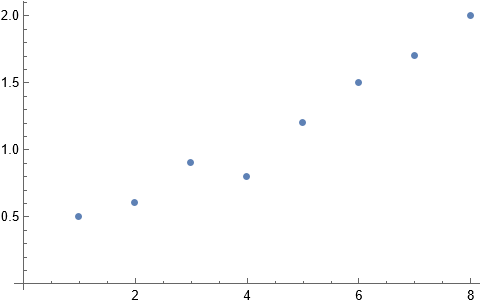
\includegraphics[width=0.75\textwidth]{grafico1.png} % Apenas o nome da imagem aqui
\subsubsection*{a)}
\noindent Para realizarmos o M.M.Q. para ajuste linear de curvas, precisamos encontrar $\alpha$ tal que $y_i = \alpha_1x_{i1} + \alpha_2x_{i2} + \dots + \alpha_px_{ip}$.
Como o \(a\) exige ajuste linear ($y = \alpha_1 x + \alpha_0 $), precisamos encontrar o ajuste de valores mínimos para a matriz gerada por $\alpha$.
\hfill\break
\hfill\break
Inicialmente, temos que:
\hfill\break
\hfill\break
$x_{i1} = x, x_{i2} = 1$. Portanto, podemos criar uma tabela que descreve o comportamento de $x_{i1}$ e $x_{i2}$ para nosso \textit{scatterplot}. 
\begin{table}[h!]
    \centering 
    \begin{tabular}{@{}ccc@{}}
    \toprule
    \textbf{$x_{i1}$} & \textbf{$x_{i2}$} & \textbf{$f$} \\ \midrule
    1                 & 1                 & 0.5          \\
    2                 & 1                 & 0.6          \\
    3                 & 1                 & 0.9          \\
    4                 & 1                 & 0.8          \\
    5                 & 1                 & 1.2          \\
    6                 & 1                 & 1.5          \\
    7                 & 1                 & 1.7          \\
    8                 & 1                 & 2.0         
    \end{tabular}
    \caption{Tabela de dados para ajuste linear}
    \label{tab:dados}
\end{table}
\hfill\break
\hfill\break
\hfill\break
\hfill\break
Com a tabela montada, podemos, então, montar nossa equação para resolução do nosso ajuste linear.
\hfill\break
\hfill\break
\[
\begin{bmatrix}
\langle \bar{x}_{i1}, \bar{x}_{i1} \rangle & \langle \bar{x}_{i1}, \bar{x}_{i2} \rangle \\
\langle \bar{x}_{i2}, \bar{x}_{i1} \rangle & \langle \bar{x}_{i2}, \bar{x}_{i2} \rangle 
\end{bmatrix}
\begin{bmatrix}
    \alpha_1 \\
    \alpha_2 
\end{bmatrix}  
=
\begin{bmatrix}
\langle \bar{f}, \bar{x}_{i1} \rangle \\
\langle \bar{f}, \bar{x}_{i2} \rangle 
\end{bmatrix}
\]

\noindent Temos:\hfill\break\hfill\break
$\langle \bar{x}_{i1}, \bar{x}_{i1} \rangle = 204$\hfill\break
$\langle \bar{x}_{i1}, \bar{x}_{i2} \rangle = 36$\hfill\break
$\langle \bar{x}_{i2}, \bar{x}_{i2} \rangle = 8$\hfill\break
$\langle \bar{x}_{i2}, \bar{x}_{i1} \rangle = 36$\hfill\break
$\langle \bar{f}, \bar{x}_{i1} \rangle = 50.5$\hfill\break
$\langle \bar{f}, \bar{x}_{i2} \rangle = 9.2$\hfill\break
\[
\begin{bmatrix}
204 & 36 \\ 
36 & 8 
\end{bmatrix}
\begin{bmatrix}
    \alpha_1 \\ 
    \alpha_2 
\end{bmatrix}  
=
\begin{bmatrix}
50.5 \\ 
9.2 
\end{bmatrix}
\]
A solução para \(\alpha_1\) e \(\alpha_2\) é dada por:

\[
\alpha = 
\begin{bmatrix}
0.217 \\
0.175
\end{bmatrix}
\]
E, portanto:
\[
f(x) = 0.217 \cdot x_1 + 0.175
\]
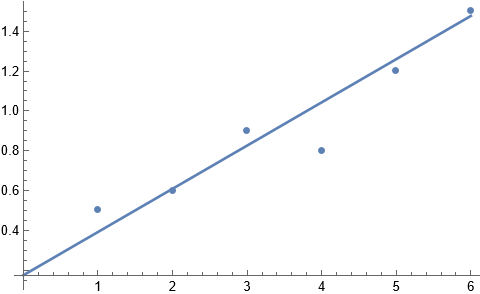
\includegraphics[width=0.75\textwidth]{grafico2.png}
\subsubsection*{b)}
A questão \(b\) exige ajuste quadrático ($y = \alpha_2 x^2 + \alpha_1 x + \alpha_0 $), precisamos encontrar o ajuste de valores mínimos para a matriz gerada para $\alpha$.
A matriz de produtos internos para uma função quadrática é dada por:

\[
\begin{bmatrix}
\langle \bar{x}_{i1}^2, \bar{x}_{i1}^2 \rangle & \langle \bar{x}_{i1}^2, \bar{x}_{i2} \rangle & \langle \bar{x}_{i1}^2, 1 \rangle \\
\langle \bar{x}_{i2}, \bar{x}_{i1}^2 \rangle & \langle \bar{x}_{i2}, \bar{x}_{i2} \rangle & \langle \bar{x}_{i2}, 1 \rangle \\
\langle 1, \bar{x}_{i1}^2 \rangle & \langle 1, \bar{x}_{i2} \rangle & \langle 1, 1 \rangle 
\end{bmatrix}
\begin{bmatrix}
\alpha_1 \\ 
\alpha_2 \\ 
\alpha_3 
\end{bmatrix}
=
\begin{bmatrix}
\langle \bar{f}, \bar{x}_{i1}^2 \rangle \\ 
\langle \bar{f}, \bar{x}_{i2} \rangle \\ 
\langle \bar{f}, 1 \rangle 
\end{bmatrix}
\]
Temos:\hfill\break\hfill\break
$\langle \bar{x}_{i1}^2, \bar{x}_{i1}^2 \rangle = 8772$\hfill\break
$\langle \bar{x}_{i1}^2, \bar{x}_{i2} \rangle = 1296$\hfill\break
$\langle \bar{x}_{i1}^2, 1 \rangle = 204$\hfill\break
$\langle \bar{x}_{i2}, 1 \rangle = 36$\hfill\break
$\langle \bar{x}_{i2}, \bar{x}_{i2} \rangle = 204$\hfill\break
$\langle 1, 1 \rangle = 8$\hfill\break
$\langle \bar{f}, \bar{x}_{i1}^2 \rangle = 319.1$\hfill\break
$\langle \bar{f}, \bar{x}_{i2} \rangle = 50.5$\hfill\break
$\langle \bar{f}, 1 \rangle = 9.2$\hfill\break
\hfill\break
E, portanto:
\hfill\break
\[
\begin{bmatrix}
8772 & 1296 & 204 \\
1296 & 204 & 36 \\
204 & 36 & 8 
\end{bmatrix}
\begin{bmatrix}
\alpha_1 \\ 
\alpha_2 \\ 
\alpha_3 
\end{bmatrix}
=
\begin{bmatrix}
319.1 \\ 
50.5 \\ 
9.2 
\end{bmatrix}
\]
\hfill\break\hfill\break
A solução para \(\alpha_1\), \(\alpha_2\) e \(\alpha_3\) é dada por:
\[
\alpha =
\begin{bmatrix}
0.015 \\
0.077 \\
0.407 
\end{bmatrix}
\]
\[
f(x) = 0.015 \cdot x^2 + 0.077 \cdot x + 0.407
\]
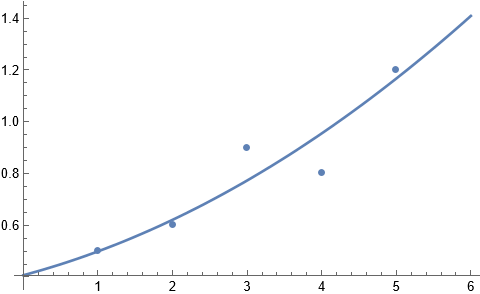
\includegraphics[width=0.75\textwidth]{grafico3.png}

Por último, precisamos calcular o resquício:
\begin{table}[h!]
    \centering
    \caption{Valores do ajuste quadrático e diferenças em relação aos valores observados}
    \begin{tabular}{ccccccccc}
        \hline
        \multicolumn{1}{c|}{$x$} & 1 & 2 & 3 & 4 & 5 & 6 & 7 & 8 \\ \hline
        $\gamma(x)$ & 0.499 & 0.621 & 0.773 & 0.955 & 1.167 & 1.409 & 1.681 & 1.983 \\
        $f(x) - \gamma(x)$ & 0.001 & 0.020 & 0.127 & 0.155 & 0.032 & 0.100 & 0.019 & 0.017 \\ \hline
    \end{tabular}
    \label{tab:ajuste_quadratico}
\end{table}
\[
\text{Somatório das diferenças quadráticas:} \quad \sum (f(x) - \gamma(x)) = 0.464
\]

\end{document}